\chapter{Diseño e implementación}
\label{cap:diseñoeimplementación}


En este capítulo abordaremos los detalles técnicos de nuestra aplicación Blind Bit. Esta aplicación está diseñada como un modelo cliente-servidor, en la que el cliente (dispositivo móvil) se encarga de solicitar los datos necesarios (origen, destino, posición actual, etc.) al usuario para enviárselos al servidor, quien calculara la ruta y responde con la guía correspondiente. De esta manera, nuestra aplicación está mejor organizada, es más eficiente y evita que los dispositivos móviles se queden sin batería rápidamente a causa de una pesada carga computacional.

Al igual que la aplicación este capítulo se divide en dos partes. La primera de ellas, Sección \ref{sec:servidor}, expone el funcionamiento general del servidor (Sección \ref{sub:func_servidor}) así como la implementación de sus dos funcionalidades principales: el cálculo de la ruta óptima (Sección \ref{sub:rutaOptima}) y la generación de instrucciones (Sección \ref{sub:genInstruc}). La segunda, Sección \ref{sec:cliente}, se centra en la implementación y el diseño de la aplicación móvil. En la Sección \ref{sub:diseño} revisamos la interfaz de la aplicación y la justificación de su diseño, mientras que en la Sección \ref{sub:func_cliente} nos adentramos en su funcionamiento desde el punto de vista técnico.

%Hemos planteado la aplicación como un modelo cliente-servidor, en la que el cliente (dispositivo móvil) se encarga de la conexión con el usuario, es decir, se ocupa de solicitar los datos necesarios (origen, destino, posición actual, etc.) para enviárselos al servidor. En ese momento el servidor resuelve el posicionamiento y procede al cálculo de la ruta (obtención de la lista de cuadrantes y de instrucciones). Una vez que el servidor ha generado esta información, vuelve a conectarse con el cliente para devolvérsela y que sea este quien finalmente se la comunique al usuario. De esta manera, nuestra aplicación está mejor organizada, es más eficiente y evita que los dispositivos móviles se queden sin batería rápidamente a causa de una pesada carga computacional. A continuación detallaremos el diseño y los detalles técnicos de la implementación tanto del cliente como del servidor.


\section{Servidor}
\label{sec:servidor}
El servidor constituye una parte indispensable del proyecto ya que se encarga de realizar los cálculos más pesados para no sobrecargar al dispositivo móvil. Sus principales funcionalidades son:
\begin{itemize}
	\item Almacenar la estructura e información referente al edificio mapeado.
	\item Permanecer a la escucha de cualquier cliente que solicite conexión.
	\item Solventar el posicionamiento del cliente conectado.
	\item Generar la ruta óptima desde la posición actual hasta el destino indicado por el cliente.
\end{itemize} 

La aplicación servidor está diferenciada en dos partes: el código escrito en lenguaje Java y los archivos correspondientes al edificio que se mapea, en nuestro caso la Facultad de Informática de la UCM. Estos archivos son los xml mencionados en la Sección \ref{sec:mapeo} y un archivo json que contiene la información referente a los distintos cuadrantes asociados a los destinos considerados por nuestra aplicación (por ejemplo, secretaría, conserjería, cafetería, las aulas,  etc.). 
Buena parte del código que conforma el servidor ha sido reutilizado de trabajos anteriores, concretamente de los proyectos de TFG \textit{Generador interactivo de instrucciones de guía sobre plataformas móviles} \citep{TFGguia} y del proyecto \textit{Sistema de guía por voz en interiores} \citep{TFGMariana}. La estructura de nuestro servidor se corresponde con la de \cite{TFGguia}. Sin embargo, hemos introducido cambios notorios para el desarrollo de esta aplicación que comentaremos a continuación.

\subsection{Funcionamiento del servidor}
\label{sub:func_servidor}

Para entender mejor la estructura del servidor, haremos un recorrido desde la carga de la información procedente de los archivos xml que representan el mapeo del edificio hasta la conexión con el cliente y el cálculo de la ruta: 


\begin{figure}[t]
	\centering
	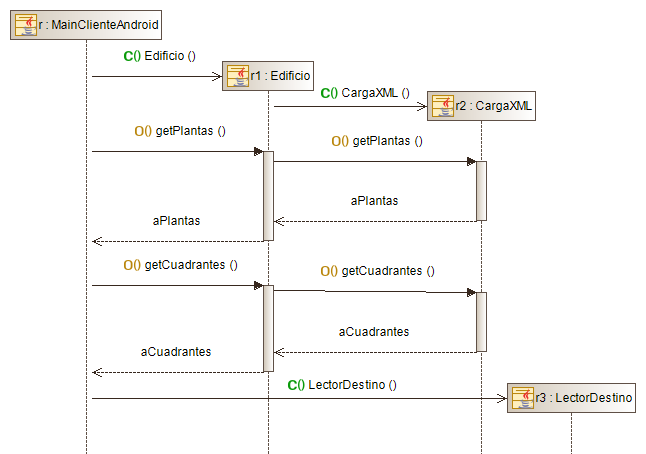
\includegraphics[width=0.8\textwidth]{Imagenes/Capitulo4/diagramasUML/arranqueServidor}
	\caption{Diagrama de secuencia para el arranque del servidor.}
	\label{fig:diag_sec_arranqueServ}
\end{figure}



\begin{itemize}
	\item \textit{Arranque del servidor:} Cuando el servidor arranca es necesario que guarde la información relativa al edifico para que pueda almacenar su estructura y generar una ruta válida para proporcionársela al cliente que la solicita. Al igual que los xml, el código relacionado con la carga de estos archivos, que conforma las clases \textit{CargaXML} y \textit{Edificio}, también se apoya en el del proyecto de \cite{TFGguia} ya mencionado en otras ocasiones. Estas clases permiten cargar los archivos y almacenar la información referente a los cuadrantes estructurada en plantas. En la Figura \ref{fig:diag_sec_arranqueServ} puede verse el diagrama de secuencia correspondiente a las explicaciones que siguen.
	
	Para nuestro trabajo se han añadido los atributos de clases necesarios para guardar la información nueva incluida en los xml (como los \textit{beacons}, los metros que ocupa el cuadrante, los pesos asociados a las conexiones, la ubicación del punto de interés o la información relevante de este) y se han eliminado aquellas que ya no se utilizan (como las coordenadas sureste y noroeste que no están presentes en nuestro proyecto). Una vez que está cargada esta información y ya tenemos la lista de cuadrantes existentes, pasamos a generar la matriz de adyacencia de la clase \textit{ListaCuadrantes} con la que representamos el mapa en forma de grafo y establecemos las conexiones entre cuadrantes. Esta tarea es relativamente sencilla, pues los xml nos proporcionan la información sobre los cuadrantes colindantes. El cambio más notorio que se ha introducido en este punto es dotar a las conexiones de la matriz de adyacencia de determinados pesos según la adaptabilidad de la ruta a nuestros usuarios objetivo. Estos cambios aparecen explicados con detalle en la Sección \ref{sub:rutaOptima}. 
	
	Es en este momento inicial cuando el servidor también carga el archivo \textit{destinos.json} con la lista de destinos y los cuadrantes asociados correspondientes. Una de sus entradas es, por ejemplo: \{``lugar'': ``aula 5'', ``cuadrante'': ``6''\}. En la clase \textit{LectorDestino} (reutilizada del proyecto de TFG \citep{TFGguia}) se almacenan cada una de las entradas en una tabla hash que cuenta con un campo clave de tipo String y un campo valor de tipo Integer que relaciona el lugar con su cuadrante asociado. 
	
	\begin{figure}[t]
		\centering
		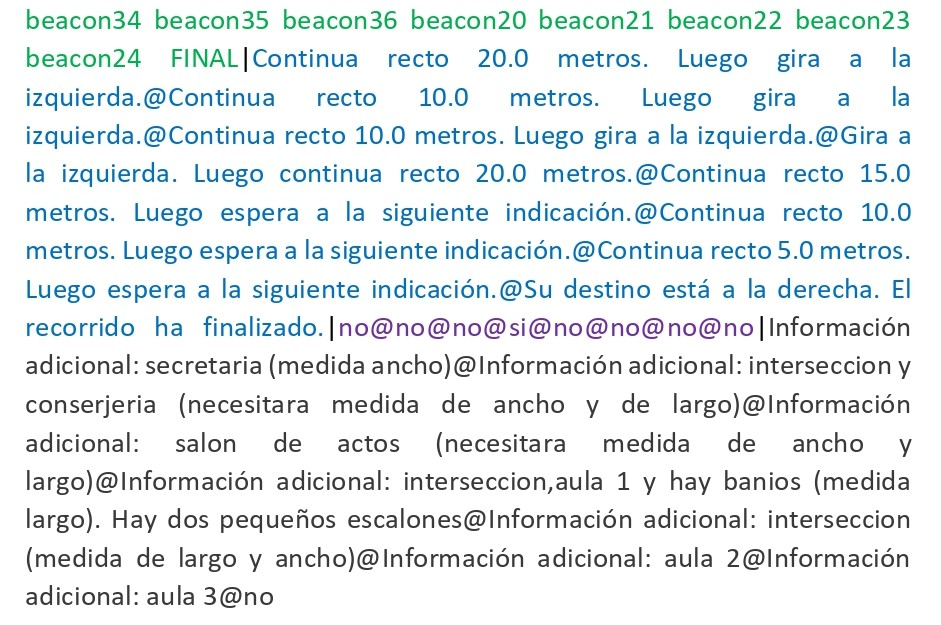
\includegraphics[width=0.9\textwidth]{Imagenes/Capitulo4/ejemploRuta}
		\caption{Ejemplo de la información generada por el servidor para una ruta desde el cuadrante $14$ al $4$.}
		\label{fig:ejemplo_ruta}
	\end{figure}
	
	\item \textit{Conexión con el cliente:} Una vez que el servidor ha almacenado toda la información correspondiente al edificio está preparado para recibir peticiones de los clientes. El servidor queda entonces a la espera de los clientes en la clase \textit{MainClienteAndroid}, escuchando a través de un \textit{webSocket} en un puerto determinado. Esta conexión cliente-servidor constituye otro de los cambios principales realizados con respecto a \cite{TFGguia}, pues se ha reestructurado por completo. En primer lugar, la conexión ya no se hace por medio de \textit{sockets} sino por medio de \textit{webSockets}. Esto implica una mayor seguridad en el intercambio de mensajes (se emplea el protocolo http) y permite que el código del servidor pueda ser utilizado como servidor externo. En nuestro caso hemos montado el servidor sobre una máquina virtual con una IP pública de la Facultad de Informática utilizando TomCat\footnote{\url{http://tomcat.apache.org/}}. Esto permite que los clientes puedan acceder al servidor desde cualquier red, lo cual es primordial para poder establecer conexión con el servidor desde la propia Facultad, en particular. En segundo lugar, el número de conexiones que tiene que establecer el cliente con el servidor para obtener la información necesaria de la ruta se ha optimizado al máximo. En un solo mensaje el servidor envía al cliente toda la información necesaria. En el proyecto que hemos tomado como modelo, el cliente, en cambio, debía solicitar al servidor una nueva instrucción cada vez que actualizaba su posición. Ahora el cliente hace una única petición indicando su \textit{beacon} más cercano (que se tomará como origen) y el destino al que quiere ir, en un mensaje del tipo \textit{IDdelBeaconOrigen$|$destino}, por ejemplo ``\textit{CPne$|$aula 8}''. Cuando el servidor recibe este mensaje, se encarga de generar la ruta desde el origen hasta el destino y enviársela al cliente. La información que se envía está compuesta por la lista de \textit{beacons} asociados a los cuadrantes que conforman la ruta desde el origen hasta el destino, las instrucciones necesarias, una lista de \textit{booleanos} que indican cuándo hay que hacer un giro en la ruta y la información adicional de los cuadrantes que conforman la ruta. Por ejemplo, para la petición del cliente \textit{beacon14$|$aula 3}, donde suponemos que \textit{beacon14} se encuentra en el cuadrante $14$ y que el aula 3 es el cuadrante 4 (ver Figura \ref{fig:ruta_optima}, línea verde), obtendríamos el mensaje que vemos en la Figura \ref{fig:ejemplo_ruta}. La lista de \textit{beacons} se representa en verde con un centinela FINAL que indica que en el \textit{beacon4} se termina la ruta, la lista de instrucciones a seguir en azul, separadas por el carácter @ atendiendo al cuadrante al que pertenecen. Debido a la imposibilidad de ir a la Facultad de Informática a causa de la COVID-19 se ha supuesto que todos los cuadrantes miden cinco metros, aunque esta información no se corresponde con la realidad. En morado se representa el cuadrante en el que hay que girar, como vemos el ``si'' corresponde al cuadrante $20$, que es en el que hay que hacer el giro. Por último, en gris se presenta la información adicional de cada cuadrante, donde un ``no'' indica que no hay información asociada a dicho cuadrante. %HAY QUE PONER AQUÍ UNA RUTA IGUAL MÁS CHULA CON LA INFORMACIÓN BIEN PERO PARA QUE SE VEA LO QUE HACE DE MOMENTO.
	
	  
	\item \textit{Generación de la ruta:} Esta funcionalidad es la más importante del servidor. El objetivo es obtener toda la información referente a la ruta desde el origen al destino seleccionado (ver Figura \ref{fig:ejemplo_ruta}). Lo primero que hay que hacer es obtener los cuadrantes origen y destino, recordemos que lo que tenemos es el \textit{beacon} más cercano al cliente y el destino como cadena de caracteres (String), pero se desconoce a qué cuadrantes corresponden. Para ello, se busca el cuadrante asociado al \textit{beacon} y al destino recorriendo la lista de cuadrantes del edificio (\textit{aCuadrantes}) y solicitando el valor asociado al destino (clave) en la tabla hash (\textit{lectorDest}). Con esta asociación entre \textit{beacons}/destinos y cuadrantes se resuelve el problema del posicionamiento. 
	
	Una vez se tienen los puntos que determinan la ruta se genera la lista de cuadrantes y de \textit{beacons} correspondientes mediante la función \textit{calculaRuta}. Esta está basada en el algoritmo de \textit{Dijkstra} (que reemplaza a la búsqueda en anchura utilizada en el proyecto de \cite{TFGguia}) que tiene como entrada la matriz de adyacencia de los cuadrantes (en la Sección \ref{sub:rutaOptima} pueden verse algunos detalles). Una vez que tenemos la lista de cuadrantes por los que el usuario debe pasar hasta llegar al destino se generan las instrucciones necesarias para guiar al usuario. Este es el cometido principal de la función \textit{generar}. Esta función tiene como entradas el cuadrante actual (en el que se encuentra el usuario), que se va simulando mediante un bucle, y el destino, y en función de los cuadrantes de la ruta, más concretamente de los inmediatos al cuadrante actual, construye la siguiente instrucción (ver detalles en la Sección \ref{sub:genInstruc}). En la Figura \ref{fig:diag_sec_conexionYRutaServ} puede verse el diagrama de secuencia.	Cuando se ha llamado a \textit{generar} con todos los cuadrantes que conforman la ruta, ya se tiene la lista de instrucciones completa y se contesta al cliente. 
\end{itemize}




\begin{figure}[t]
	\centering
	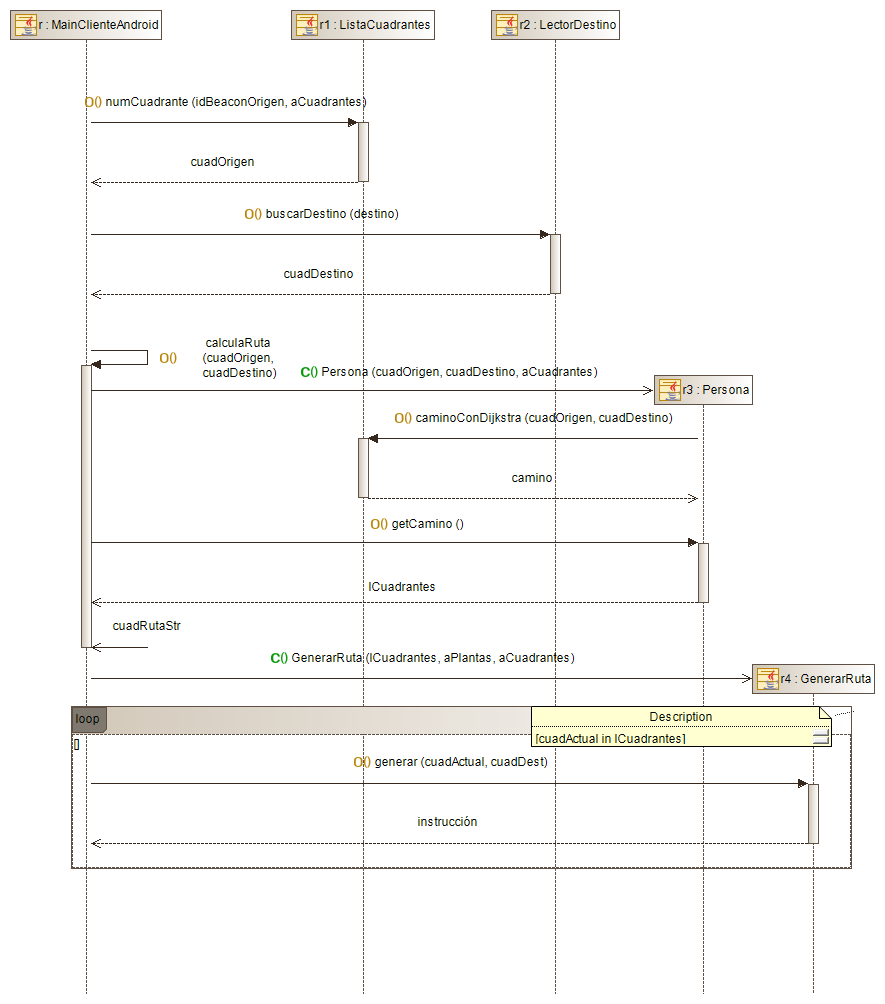
\includegraphics[width=0.8\textwidth]{Imagenes/Capitulo4/diagramasUML/generacionRuta}
	\caption{Diagrama de secuencia para la generación de la ruta.}
	\label{fig:diag_sec_conexionYRutaServ}
\end{figure}



\subsection{Cálculo de la ruta óptima}
\label{sub:rutaOptima}

En esta sección veremos las modificaciones que se han hecho para lograr guiar al usuario por la ruta más conveniente. Como ya hemos mencionado anteriormente, el mapeo nos proporciona un grafo en el que los cuadrantes son los nodos y las conexiones entre ellos, las aristas. Para su representación hemos empleado una matriz de adyacencia y de esta manera el cálculo de la ruta más corta entre dos cuadrantes se reduce al algoritmo de \textit{Dijkstra}.

Sin embargo, no debemos olvidar que nuestra aplicación tiene un usuario final muy concreto: personas con discapacidad visual. Es por ello que la ruta debe ser lo más sencilla posible, libre de obstáculos y otros elementos que puedan entorpecerlos, por lo que en ocasiones la ruta óptima no coincide con la más corta sino con la que esté mejor adaptada. Para representar esta adaptabilidad, a aquellas conexiones que presenten una mayor dificultad para las persona invidentes se les ha asignado un peso mayor en la matriz de adyacencia (ver Sección \ref{sub:mapeo_xml}), a fin de buscar este equilibrio entre la ruta más corta y la más adecuada. En la Figura \ref{fig:ruta_optima} aparece un ejemplo de esta situación: si quisiéramos ir desde la puerta principal (cuadrante $14$) al aula 3 (cuadrante $4$), el camino más corto implicaría pasar por delante de los ascensores (ruta roja). Sin embargo, la conexión entre los cuadrantes $11$ y $12$, y $2$ y $11$ puede resultar tediosa para una persona invidente. Las razones que hemos considerado son: 
\begin{itemize}
	\item El tramo compuesto por los cuadrantes $2$, $11$ y $12$ es más estrecho que su camino paralelo por el \textit{hall}.
	\item Presenta más giros e intersecciones de caminos.
	\item Normalmente acumula más gente ya que es zona de paso para coger los ascensores o subir/bajar por las escaleras o entrar/salir de la cafetería.
\end{itemize} 
 	Todo esto es potencialmente problemático en ausencia de la vista y considerando además que nuestros usuarios es probable que vayan acompañados de un perro guía o un bastón. Por ello, hemos concluido ajustar los pesos en la matriz de adyacencia y la ruta generada pasa a ser la señalada en verde. De esta manera limitamos el paso por el pasillo de los ascensores a aquellas rutas en las que es estrictamente necesario, es decir, cuando se requiere un cambio de planta. Este tipo de consideraciones se han tenido en cuenta en las distintas zonas del edificio que presentan este tipo de características.


\begin{figure}[t]
	\centering
	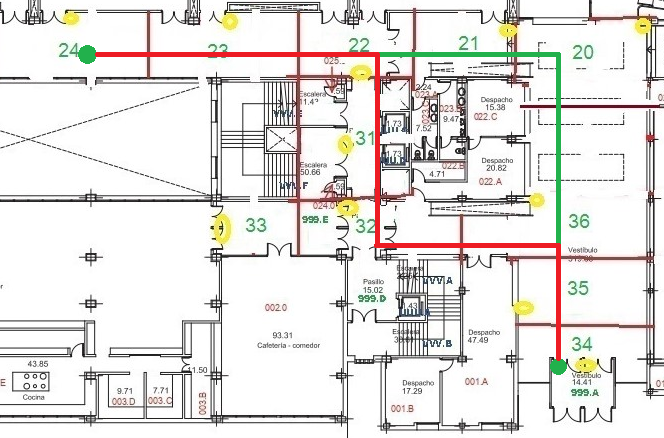
\includegraphics[width=0.8\textwidth]{Imagenes/Capitulo4/mapa_ruta_optima}
	\caption{Ejemplo de ruta óptima entre dos puntos.}
	\label{fig:ruta_optima}
\end{figure}

\subsection{Generación de instrucciones}
\label{sub:genInstruc}

La función que contiene toda la lógica relativa a la generación de las instrucciones es \textit{generar}. Esta función es una de las que más modificaciones ha sufrido con respecto a los trabajos predecesores, pues no solo la hemos adaptado para personas con discapacidad visual sino que también hemos incluido mucha complejidad procedente de los cambios de planta y demás casuística que no estaba previamente incluida. Algunas de las modificaciones son: 

\begin{itemize}
	\item Se ha añadido más precisión e información a las instrucciones. De esta manera, cuando el usuario llega al destino correspondiente la instrucción especifica dónde se encuentra este, véase ``Su destino está a la derecha (o a la izquierda o delante...).'' dependiendo de por dónde haya llegado el usuario (en la Sección \ref{sub:instr_giro} se detalla la implementación de esta funcionalidad). Otro caso en el que se ha añadido mayor precisión es al puntualizar los metros que el usuario debe continuar en una dirección dada. En la Figura \ref{fig:ejemplo_ruta} podemos ver un ejemplo de ruta en el que se especifica el número de metros que el usuario debe seguir recto hasta ejecutar el siguiente giro o la siguiente acción, y como a medida que el usuario va avanzando la distancia va disminuyendo. Esto favorece que el usuario reconozca que va en la dirección correcta y pueda calcular mejor cuando ha de girar o ejecutar cualquier otra acción. A diferencia de los trabajos predecesores, nuestra app proporciona una instrucción nueva en cada cuadrante, es decir, no se salta ninguno como sucedía en el caso de las rectas (pasillos) en el proyecto precedente. Esto se ha hecho así ya que por un lado hemos considerado cuadrantes más grandes y por tanto la distancia recorrida de un cuadrante a otro es mayor, y porque creemos muy conveniente que el usuario reciba de manera continuada \textit{feedback} por parte de la aplicación para cerciorarse de que va por el camino correcto y que la aplicación no ha dejado de funcionar. Finalmente, también se ha ajustado el orden de las instrucciones para proporcionarlas de manera correcta. De modo que si la instrucción siguiente es un giro se invierte el orden para indicar primero el giro y después los metros que debe continuar en la nueva dirección.
	
	
	\item Se han incluido cambios de planta, lo qu supone una gran novedad respecto al proyecto citado \cite{TFGguia}. Ahora los cuadrantes de distintas plantas correspondientes a los ascensores están unidos\footnote{El cuadrante $11$ (correspondiente a los ascensores situados detrás de conserjería) está conectado con el $37$ (ascensor correspondiente al anterior en la planta 1) y el $9$ (ascensor más cercano a la puerta trasera de la cafetería) con el $29$ (ascensor correspondiente al anterior en la planta 1).} permitiendo así que la lista de cuadrantes de la ruta esté formada por cuadrantes de distinta planta. La función \textit{generar} detecta cuando el siguiente cuadrante al que queremos ir no está en la misma planta que el de nuestra posición actual y genera la instrucción en consonancia ``Los ascensores están a tu izquierda. Sube a la primera planta'' o ``El ascensor está delante. Sube a la primera planta'', por ejemplo. También se tiene en cuenta en las instrucciones el caso particular de las zonas de ascensores, pues hay dos zonas por planta pero no son simétricas por lo que las instrucciones son distintas. Por ello, para salir de la zona de los ascensores correspondientes al cuadrante $11$ (los que se sitúan detrás de conserjería) debemos simplemente girar, mientras que para salir de los de la zona de la puerta trasera de la cafetería (cuadrante $29$) debemos caminar escasos metros hacia adelante y después girar. A pesar de que en la Facultad de Informática contamos con ascensores y escaleras, se ha supuesto que la ruta se seguirá por medio de los ascensores ya que de esta manera es más fácil el cambio de planta y, además, estos se encuentran adaptados con botones en \textit{braille}.
	
	\item Se ha añadido una funcionalidad que permite informar al usuario (si lo desea) sobre lo que se va encontrando a su paso por la ruta, véase los baños, la cafetería, el despacho de Delegación de Alumnos, unos escalones, etc. Esto es fundamental pues además de proporcionar seguridad al usuario en su primera visita a un edificio, le da la opción de tener una mejor idea global del espacio en el que se encuentra. Para ello lo que se hace es incluir en la ruta la información contenida en el cuadrante siguiente al que se encuentra el usuario, de esta manera conseguimos adelantarnos y avisar al usuario con antelación. Así mismo, la función \textit{generar} enviará información sobre cuándo el usuario deberá hacer un giro para permitir avisar a este de manera especial (con una vibración) desde la aplicación del cliente.
	
\end{itemize}

\begin{figure}[t]
	\centering
	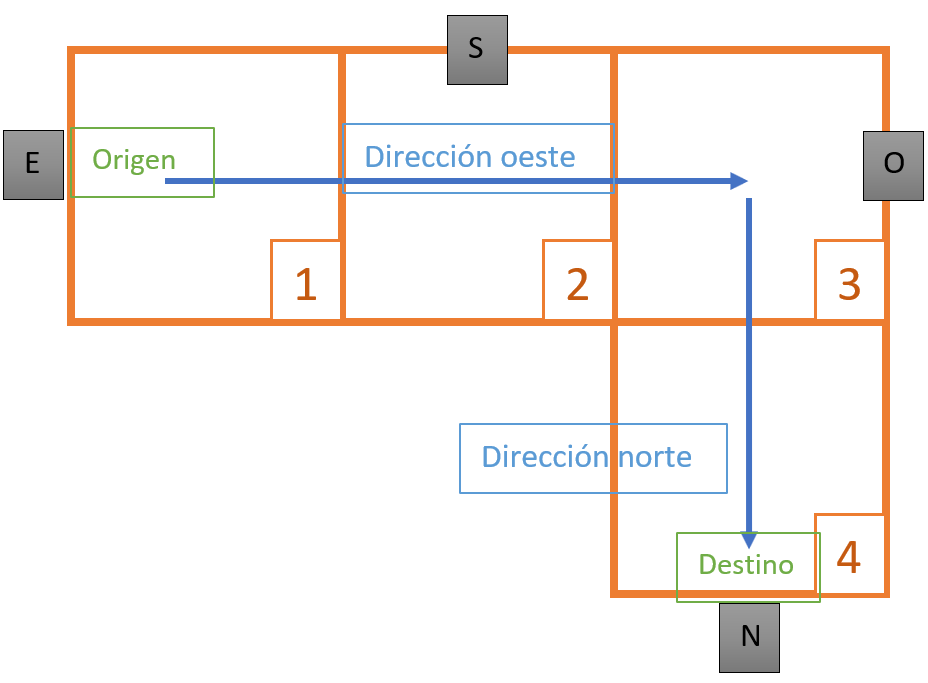
\includegraphics[width=0.8\textwidth]{Imagenes/Capitulo4/simulacion_giro}
	\caption{Ejemplo de giro en la ruta.}
	\label{fig:simulacion_giro}
\end{figure}


\subsubsection{Implementación de las instrucciones de giro}
\label{sub:instr_giro}

Como ya avanzábamos al comienzo de la sección anterior, la función que genera las instrucciones completas es \textit{generar}. Sin embargo, esta se apoya en la función \textit{indicaDirFinal}, cuya finalidad es indicar si se debe hacer un giro y, en ese caso, hacia qué lado. Esto resulta de gran utilidad tanto para saber hacia dónde debe dirigirse el usuario en caso de que tenga que hacer un cambio de dirección en su camino como para poder indicarle dónde se encuentran ciertos puntos de interés durante la ruta, (como los ascensores o el destino) si a su izquierda, a su derecha o delante.

La lógica de la función \textit{indicaDirFinal} es bastante sencilla. Esta toma como parámetro de entrada dos direcciones, la primera de ellas indica la dirección en la que vamos y la segunda la dirección a la que queremos llegar. En la Figura \ref{fig:simulacion_giro} se ilustra el ejemplo de una ruta con un giro. En este caso, la dirección en la que vamos sería el oeste (en gris se muestra la posición de los puntos cardinales de referencia). Al llegar al cuadrante $3$, la dirección que debemos tomar es norte, la cual no coincide con la dirección que llevábamos. Es entonces cuando la función \textit{generar} sabe que el usuario debe hacer un giro y llama a la función \textit{indicaDirFinal} con los parámetros oeste y norte, en ese orden. La lógica de \textit{indicaDirFinal} se basa en una serie de \textit{if-elses} que determinan las direcciones de giro correspondientes. En este caso en el cuadrante $3$ nos devolvería el giro a la derecha. Una vez que nos encontramos ya en el cuadrante $4$, \textit{generar} reconoce que es el cuadrante destino (pues este uno de sus parámetros de entrada) y, en función de dónde se sitúe el punto de interés de este cuadrante destino, indica al usuario dónde está con ayuda de la función \textit{indicaDirFinal}. En este caso sería \textit{su destino está delante}, pues no hay que realizar ningún cambio de dirección. 



%Comento la figura del diagrama de clases porque quiero ver cómo lo reorganizo
%\begin{figure}[t]
%	\centering
%	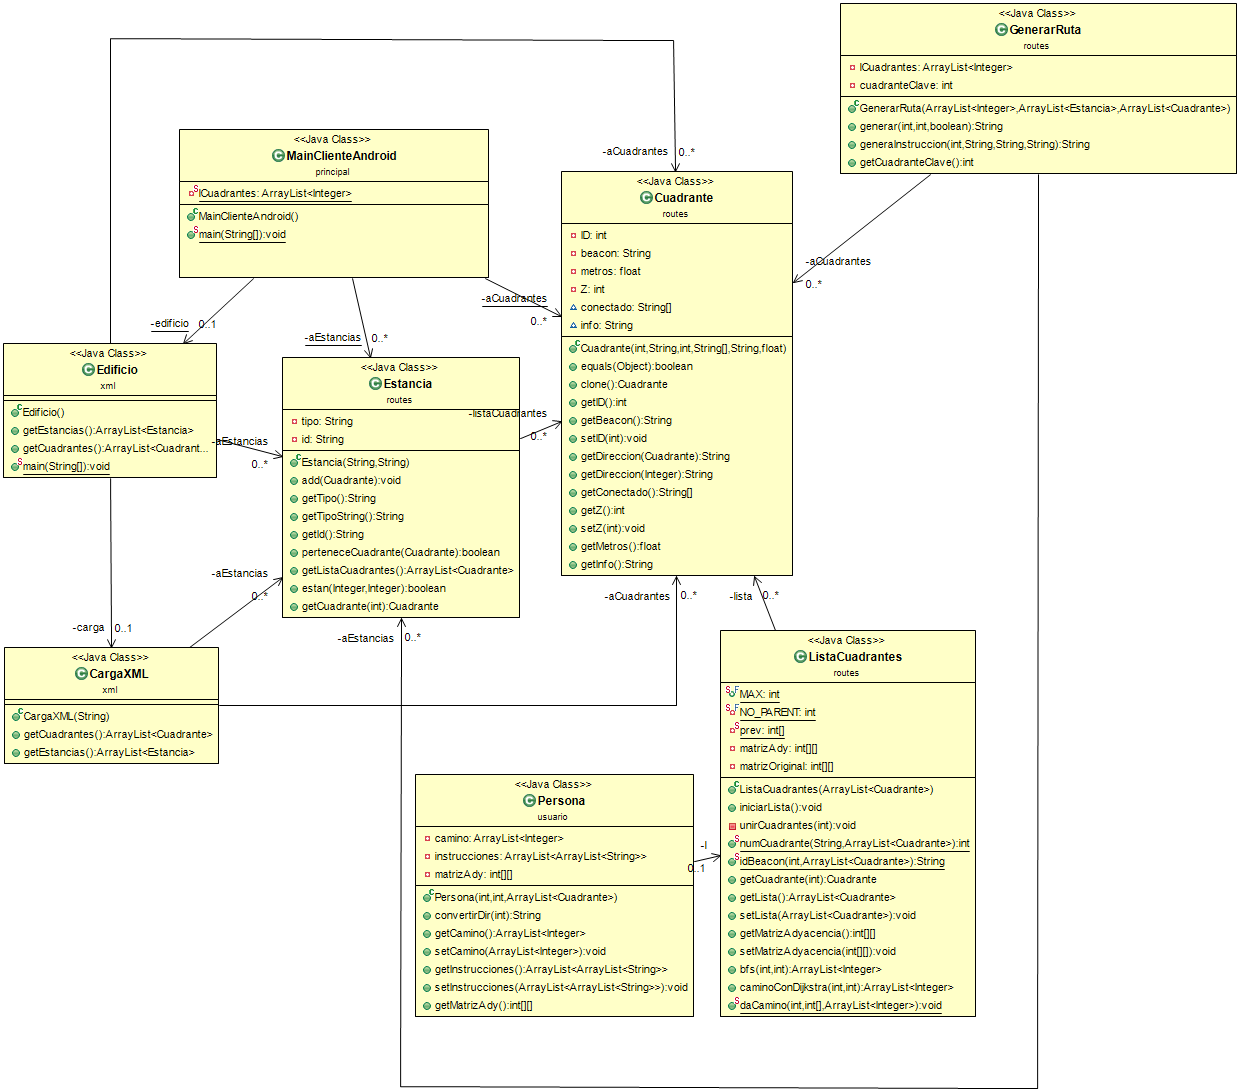
\includegraphics[width=1.1\textwidth]{Imagenes/Capitulo4/diagramServer}
%	\caption{Diagrama de las clases principales del servidor.}
%	\label{fig:diagServ}
%\end{figure}



\section{Cliente}
\label{sec:cliente}
En nuestro proyecto el cliente constituye la aplicación en sí misma. Esta la hemos bautizado como Blind Bit y ha sido desarrollada para Android. A través de ella el usuario solicita la ruta a un destino determinado, la aplicación conecta entonces con el servidor, que es quien la calcula, y se la reenvía al cliente. Finalmente, la aplicación se encarga de proporcionar, en el momento adecuado, las instrucciones necesarias para llegar al destino y utiliza sonidos y vibraciones para advertir de diferentes situaciones, como giros o aprobación de que seguimos en el camino correcto.

El cliente está desarrollado como un código genérico que es completamente independiente al edificio que se refiere. De esta manera, puede reutilizarse siempre que se incluya la información pertinente siguiendo el modelo que planteamos. La información a incluir es aquella relativa a la lista de destinos que la guía es capaz de reconocer y ha de ubicarse en el archivo XML \textit{listasStringsApp.xml}. En este archivo se encuentran los destinos con el mismo nombre que a su vez reconoce el servidor y que incluye respectivamente en el archivo \textit{destinos.json}, lo que permite que antes de conectar con el servidor podamos comprobar que el destino solicitado por el usuario es correcto. %También habría que modificar esta lista de destinos en las instrucciones de uso de la aplicación para que el usuario pueda acceder a ella sin necesidad de tener que simular el inicio de una ruta.

A continuación presentamos tanto los detalles de diseño de la aplicación como los detalles técnicos de su implementación.

\subsection{Diseño de la aplicación Blind Bit}
\label{sub:diseño}

A la hora de abordar el diseño de la aplicación hemos tenido muy presente el hecho de que nuestros potenciales usuarios finales son personas con discapacidad visual. Por ello hemos plateado interfaces sencillas y poco aglomeradas, en las que los botones sean lo más grandes posibles y estén bien organizados para que sea fácil de utilizar y memorizar. De esta manera, la mayor parte de los botones que hemos incluido tienen forma rectangular y ocupan todo el ancho de la pantalla, lo que favorece el uso de la app con ayuda del lector de pantalla. No solo hemos tenido en cuenta el lector de pantalla en la forma y el tamaño de los botones sino también a la hora de cambiar el nombre de cada pantalla especificando en cual se encuentra el usuario (por defecto aparecía el mismo nombre en todas) y en el hecho de evitar que este reproduzca todas las figuras que aparecen en la pantalla (modo por defecto) ya que sobrecarga al usuario proporcionándole información que en algunos casos carece de interés, como sucede con el logotipo de la app o ciertos cuadros de texto.

Por otro lado, hemos incluido algunas vibraciones y sonidos característicos con el fin de advertir al usuario de ciertas situaciones y acciones de manera no verbal. De esta manera, no saturamos al usuario con demasiada información extra pero le ayudamos en el uso de la app. Estos son: sonido de \textit{acierto} cuando el usuario completa correctamente la instrucción dada, una vibración larga en el momento en el que pasa por una intersección de caminos y ha de girar a la izquierda, dos vibraciones cortas cuando en cambio ha de girar a la derecha y tres cuando ha llegado a su destino.

A continuación describimos las pantallas de nuestra aplicación, que pueden verse en la Figura \ref{fig:interfaz}, y los detalles de su diseño:

\begin{figure}
	\def\tabularxcolumn#1{m{#1}}
	\centering
	\begin{tabularx}{\linewidth}{@{}cXX@{}}
		%
		\begin{tabular}{ccc}
			\subfloat[Pantalla principal]{\includegraphics[width=0.3\textwidth]{Imagenes/Capitulo4/PantallaPrincipal}} 
			& \subfloat[Pantalla de destinos]{\includegraphics[width=0.3\textwidth]{Imagenes/Capitulo4/PantallaListaDestinos}}
			& \subfloat[Pantalla de aulas]{\includegraphics[width=0.3\textwidth]{Imagenes/Capitulo4/PantallaListaAulas}}\\
			\subfloat[Pantalla de ruta]{\includegraphics[width=0.3\textwidth]{Imagenes/Capitulo4/PantallaRuta}} 
			& \subfloat[Pantalla instrucciones]{\includegraphics[width=0.3\textwidth]{Imagenes/Capitulo4/PantallaInstrucciones1}}
			& \subfloat[Segunda pantalla instrucciones]{\includegraphics[width=0.3\textwidth]{Imagenes/Capitulo4/PantallaInstrucciones2}}\\
			%\subfloat[E]{\includegraphics[width=0.3\textwidth]{Imagenes/Capitulo4/PantallaPrincipal}} 
			%& \subfloat[F]{\includegraphics[width=0.3\textwidth]{Imagenes/Capitulo4/PantallaPrincipal}}\\
		\end{tabular}
		%&
		%\subfloat[G]{\includegraphics[width=0.3\textwidth]{Imagenes/Capitulo4/PantallaPrincipal}}
		%&
		%\subfloat[H]{\includegraphics[width=0.3\textwidth]{Imagenes/Capitulo4/PantallaPrincipal}}
	\end{tabularx}
	
	\caption{Interfaz de la aplicación Blind Bit}\label{fig:interfaz}
\end{figure}

\begin{itemize}
	\item \textit{Pantalla principal:} En ella aparece el logo de la aplicación que ocupa el cuadro superior, y tres botones alargados que se sitúan en el cuadro inferior ocupando prácticamente todo el ancho de la pantalla. Los botones son, en orden descendente, \textit{Iniciar Ruta}, \textit{Ajustes} e \textit{Instrucciones}. La finalidad de estos botones es muy intuitiva: el botón de \textit{Iniciar Ruta} nos conduce a una pantalla de destinos en la que podremos seleccionar uno para después comenzar la ruta hasta él; el botón de \textit{Ajustes} sirve para modificar algunos aspectos de la configuración como el volumen, el idioma de la aplicación, el tipo de voz que da las instrucciones, el modo de uso de la aplicación (que de más información en las instrucciones o que sean más escuetas), ect; y por último, el botón de \textit{Instrucciones} conduce a una pantalla en la que se expone el modo de uso de la aplicación, con todas sus posibilidades.
	
	\item \textit{Pantalla de destinos:} Esta pantalla tiene como finalidad que el usuario seleccione el destino de la Facultad de Informática hasta el que quiere dirigirse para, tras ello, comenzar con la ruta. Debido al carácter especial de nuestros usuarios, hemos empleado un diseño que aporte distintas alternativas a esta búsqueda del destino pues nuestro objetivo no es solo encontrar una vía que les resulte sencilla (como podría ser utilizar la app mediante voz) sino que también se amolde a distintas situaciones de la vida cotidiana (siguiendo con el mismo ejemplo, en determinadas circunstancias utilizar la app mediante voz puede ser molesto o causar vergüenza al usuario). Por ello, en el margen superior de la pantalla hemos situado una barra de escritura, que ocupa todo el ancho, en la que el usuario puede escribir directamente el nombre del destino al que desea ir. Si por el contrario prefiere utilizar la app mediante voz hemos incluido un micrófono en la parte central del margen inferior a través del cual el usuario puede indicar el destino en voz alta. El motivo por el cual hemos decidido colocar el micrófono en la parte inferior de la pantalla es que pese a que el lector de pantalla va barriendo de arriba a abajo y, por tanto, el micrófono queda el último, ocupa una posición cercana al dedo pulgar tanto de la mano derecha como de la izquierda (ya que se ha colocado en medio) y por ende, aunque al principio haya que esperar un poco más hasta que el lector lo encuentre, una vez que el usuario sepa donde está, el acceso será más sencillo y rápido. Además no hay ningún otro botón próximo, lo que facilita aún más el acceso. Finalmente, siguiendo el modelo de diseño de la aplicación \textit{Lazarillo}, vista en la Sección \ref{sec:appGuia} del Capítulo \ref{cap:estadoDeLaCuestion}, hemos incluido una cuadrícula con 9 botones (3 filas de 3 botones) en la zona centra, en la que aparecen todos los posibles destinos de la Facultad (\textit{Aulas}, \textit{Cafetería}, \textit{Biblioteca}, \textit{Salón de Actos}, \textit{Sala de Juntas}, \textit{Sala de Grados}, \textit{Consejería},\textit{ Puerta Principal}, \textit{Secretaría}). Esta tabla se genera dinámicamente organizándose en filas de 3 botones como máximo y teniendo tantas filas como sean necesarias para incluir todos los destinos leídos del archivo \textit{listasStringsApp.xml}. Los botones se colorean intercaladamente de lila y blanco para que aquellos usuarios que tienen visibilidad reducida puedan distinguir los botones por sus colores. 
	
	Si se selecciona el botón \textit{Aulas} aparece la misma pantalla con la única variante de que la cuadrícula generada hace referencia a las aulas leídas del mismo archivo (\textit{listasStringsApp.xml}). Como en el caso concreto de la Facultad de Informática hay 16 aulas, la tabla está formada por 5 filas con 3 botones en cada una y una última fila en la que solo hay un botón. Si por el contrario se selecciona cualquier otro botón de destino (un aula concreta, la cafetería, la sala de juntas, etc.) o se indica el destino con alguna de las otras dos alternativas (barra de escritura o micrófono) aparece la pantalla de ruta.
	
	\item \textit{Pantalla de ruta:} Esta pantalla es la encargada de proporcionar las instrucciones de la ruta hasta el destino seleccionado. En ella aparece un cuadro de texto en la parte superior, en el que se van escribiendo las instrucciones a medida que se reproducen en voz alta y un botón con forma de altavoz situado encima del cuadro de texto en la parte derecha, que sirve para silenciar la reproducción de las instrucciones. Al pulsar sobre él cambia su aspecto físico y pasa a ser un altavoz con una cruz que nos indica su nuevo estado (\textit{mute}). De nuevo hemos tomado la decisión de no usar exclusivamente la vía oral con el fin de crear una aplicación que se adapte a diversas situaciones y usuarios (personas invidentes, personas con discapacidad pero que mantienen algún resto visual e incluso personas videntes que busquen una guía por la Facultad), y sea así, lo más inclusiva posible. Además del cuadro de texto, aparecen 4 botones alargados que ocupan el resto de la pantalla. Estos son \textit{Iniciar Ruta} que como su nombre indica sirve para comenzar una vez que se ha seleccionado el destino, \textit{Repetir Instrucción} cuya finalidad es volver a dar la última instrucción en caso de que no se haya escuchado bien, \textit{Instrucciones Detalladas} que sirve para activar y desactivar, según el estado previo, la funcionalidad de incluir más información durante la ruta (indicar qué hay alrededor). Cuando se modifica el estado de este botón el lector de pantalla avisa del nuevo \textit{modo instrucciones detalladas activado} o \textit{modo instrucciones detalladas desactivado}. Y por último, \textit{Finalizar Ruta} que sirve para forzar la finalización de la ruta. Cuando se pulsa este botón o bien la flecha para ir hacia atrás aparece una ventana emergente que pide confirmación para finalizar. De esta manera nos aseguramos de que el usuario no ha pulsado sin querer. 
	
	Atendiendo de nuevo a esta diversidad de usuarios, hemos coloreado los botones \textit{Iniciar Ruta} e \textit{Instrucciones Detalladas} en morado y lila respectivamente, para que aquellos que tienen visibilidad reducida puedan distinguir los botones por sus colores. Por otro lado, el motivo por el cual hay un botón de \textit{Iniciar Ruta} en lugar de empezar directamente con la reproducción de instrucciones una vez que el destino ha sido seleccionado, es que tras hacer varias pruebas con el lector de pantalla advertimos que las instrucciones y el \textit{talkback} se solapaban y se volvían ininteligibles.
	
	\item \textit{Pantalla de Instrucciones de uso:} En esta pantalla aparece el logo de la aplicación centrado en el margen superior y a continuación cuatro botones formando una columna en los que se plantean algunas de las dudas más frecuentes sobre el uso de Blind Bit: \textit{Cómo iniciar una ruta}, \textit{Cómo buscar un destino}, \textit{En qué consiste Repetir Instrucción} y \textit{Qué son las Instrucciones Detalladas}. Al pulsar cualquiera de estos botones aparece una pantalla que nos recuerda al diseño de la pantalla de ruta, en ella hay un gran cuadro de texto que ocupa la mitad superior de la pantalla y tres botones colocados en forma de columna que ocupan la otra mitad. Estos botones son, en orden descendente, \textit{Reproducir}, \textit{Siguiente} y \textit{Anterior}. De esta manera, si pulsas el primer botón (\textit{Reproducir}) aparece la instrucción correspondiente al modo de uso seleccionado, escrita en el cuadro de texto y reproducida en voz alta. Para volver a escucharla basta con pulsar de nuevo este mismo botón. Por otro lado, si se quiere saber la instrucción siguiente o anterior siguiendo el orden indicado en la pantalla de Instrucciones de uso, basta con pulsar el botón correspondiente (\textit{Siguiente} o \textit{Anterior}, respectivamente). Con respecto a las decisiones tomadas en el diseño de esta última pantalla, hemos colocado los botones en este orden ya que hemos considerado que \textit{Reproducir} será el más utilizado y por ello parece conveniente que esté arriba. Siguiendo con esta linea de pensamiento, parece que lo más lógico a continuación, es querer ir a la instrucción siguiente por lo que hemos colocado justo debajo dicho botón (\textit{Siguiente}) y por último, el botón \textit{Anterior} en caso de que querer volver a una instrucción previa. Por otro lado, al igual que en la pantalla de ruta las instrucciones no empiezan hasta que no se pulsa el botón \textit{Reproducir}. Esto se debe al mismo motivo que entonces, si se usa la app con ayuda del lector de pantalla y las instrucciones comienzan directamente, se producen solapamientos en las reproducciones y se vuelven ininteligibles.
\end{itemize}



\subsection{Funcionamiento del cliente}
\label{sub:func_cliente}
En esta sección veremos el funcionamiento de la aplicación desde la interacción con el usuario hasta la conexión con el servidor y gestión de la ruta. 

\begin{itemize}
	\item \textit{Interacción con el usuario}: Como ya hemos tratado en la Sección \ref{sub:diseño} la aplicación está diseñada para que el usuario pueda lograr el objetivo con la mínima cantidad de pasos. Tanto es así que la interacción con el usuario queda reducida al mínimo. Para iniciar una ruta tan solo se pide al usuario que introduzca el destino al que quiere ir (una vez ha pulsado \textit{Iniciar ruta} en la pantalla \textit{principal}). Esto se hace a través de la pantalla \textit{Lista de destinos}, que se pueden ver en la Figura \ref{fig:interfaz}. Cuando el usuario selecciona el destino, la aplicación abre la pantalla \textit{Ruta}, resuelve el problema de posicionamiento y espera a que el usuario pulse sobre \textit{Iniciar ruta}. En ese momento, la aplicación conecta con el servidor y comienza la ruta con instrucciones guiadas por voz.
	
	\item \textit{Posicionamiento}: En la Sección \ref{sub:conclusiones_posicionam} concluimos que el problema del posicionamiento se resolvería asignando al usuario el cuadrante correspondiente a su \textit{beacon} más cercano. La lógica que lleva a cabo este proceso está en la clase \textit{ScanningActivity}. Para ello comienza el escaneo de los \textit{beacons} con la función \textit{startScanning}. Una vez que se tiene la lista de \textit{beacons} que están en el rango de detección del dispositivo móvil del usuario, se toma el más cercano en función de la distancia estimada por la función \textit{getDistance} de la SDK de \textit{Kontakt} y, cuando el usuario pulsa sobre botón \textit{Iniciar ruta}, se conecta con el servidor para obtener los detalles de la ruta solicitada por el usuario. 
	
	
	\begin{figure}[t]
		\centering
		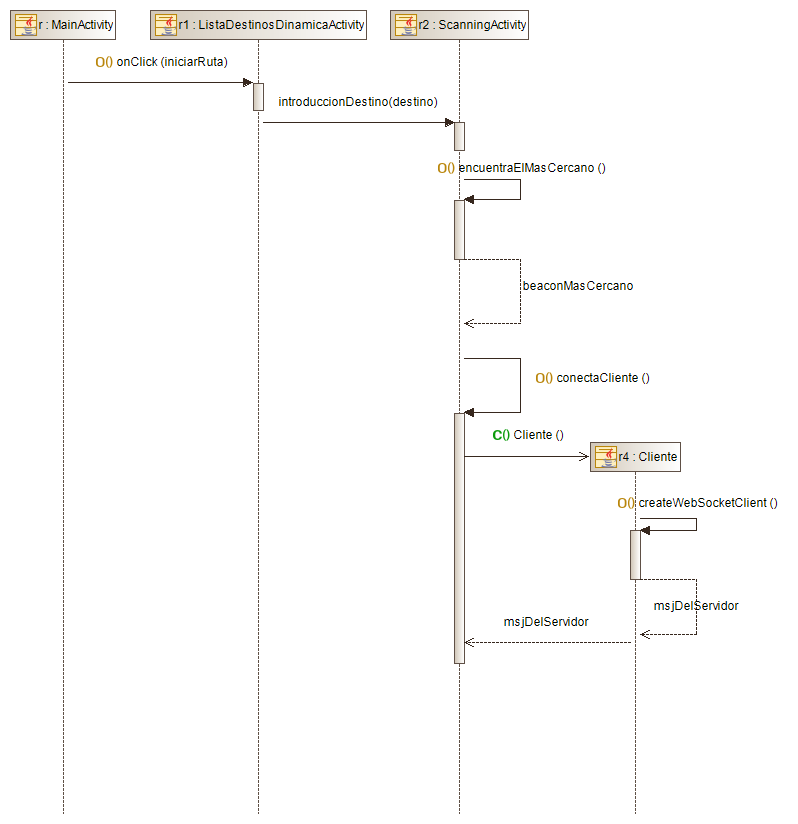
\includegraphics[width=0.8\textwidth]{Imagenes/Capitulo4/diagramasUML/clienteHastaSeguimientoRuta}
		\caption{Diagrama de secuencia que comprende la interacción con el usuario, la resolución del posicionamiento y la conexión con el servidor en el cliente.}
		\label{fig:diag_clientePrimeraParte}
	\end{figure}
		
	\item \textit{Conexión con el servidor}: El código correspondiente a esta funcionalidad se recoge en la clase \textit{Cliente}. Cuando se llama a esta clase se pasan como parámetros el \textit{beacon} más cercano y el destino al que quiere ir el usuario. Con esta información se genera un mensaje del tipo \textit{IDdelBeaconOrigen$|$destino} que se manda al servidor por medio de un \textit{webSocket}. Cuando el servidor genera la ruta manda al cliente un mensaje con toda la información referente a la ruta (ver Sección \ref{sub:func_servidor}). Este mensaje se recibe y desglosa en la lista de \textit{beacons} de la ruta, las instrucciones, la información sobre los giros y la información adicional de los cuadrantes de la ruta. Cuando tiene toda la información avisa a la aplicación (que ha quedado esperando la llegada de este mensaje) y la ejecución continua de nuevo en \textit{ScanningActivity}, donde se guarda la información de la ruta en vectores que se irán recorriendo según avance el usuario. Si no se consigue conectar con el servidor la aplicación genera un mensaje especial que se gestiona en \textit{ScanningActivity} para que la aplicación no quede en espera infinita y acabe bloqueando el dispositivo. En la Figura \ref{fig:diag_clientePrimeraParte} puede verse el diagrama de secuencia que describe las funcionalidades detalladas hasta este momento (interacción con el usuario, posicionamiento y conexión con el servidor).


	\item \textit{Seguimiento de la ruta}: Una vez que la conexión con el servidor ha tenido éxito y tenemos toda la información de la ruta almacenada en los vectores correspondientes se comienza guiar al usuario. Para ello se inicia el índice \textit{indiceRuta} a cero y se da al usuario la primera instrucción. Este índice indica en qué punto de la ruta estamos, cada vez que cambiamos de cuadrante se va incrementando en uno, siempre que estemos siguiendo la ruta. Una vez que el usuario ha recibido la primera instrucción, se va llamando a la función \textit{onEddystonesUpdated} cada dos segundos (parámetro configurable) a fin de saber en qué momento el usuario tiene como \textit{beacon} más cercano el siguiente \textit{beacon} de la ruta. Imaginemos, por ejemplo, que los dos primeros cuadrantes de la ruta fueran el $0$ y el $1$. Cuando se inicia la ruta y el usuario recibe la primera instrucción, la función \textit{onEddystonesUpdated} se dará cuenta de en qué momento el usuario tiene el \textit{beacon1} como más cercano y le dará la siguiente instrucción. Esto mismo ocurre con el resto de \textit{beacons} de la ruta, hasta llegar al final. Si la funcionalidad \textit{Instrucciones detalladas} está activada, se va proporcionando al usuario la información adicional correspondiente a su posición inmediatamente después de la instrucción que debe ejecutar.
	
	Durante la ruta el usuario percibe no solo información oral sobre las instrucciones o la información adicional de los cuadrantes (si tiene la funcionalidad \textit{instrucciones detalladas} activada), sino también percibe en el dispositivo sonidos y vibraciones. En el caso de que el usuario complete una instrucción, es decir, llegue al siguiente \textit{beacon} de la ruta, la aplicación emite un sonido \textit{check} para hacerle saber que ha completado esa parte. Además, si la instrucción siguiente es un giro, el dispositivo vibra, durante un segundo, si es un giro a la izquierda, y dos vibraciones de medio segundo, si es un giro a la derecha, para notificar el cambio de dirección. Así mismo, cuando el usuario ha llegado al final de la ruta, el dispositivo emite tres vibraciones cortas avisando de que se ha llegado al destino. Esto provoca en el usuario una sensación de control y seguridad, pues puede comprobar en tiempo real que va en el camino correcto y permite que el usuario tenga menos probabilidades de perderse, pues las notificaciones del cambio de sentido están reforzadas.
	
	Se espera que el usuario pueda llegar al destino con la guía que proporciona la aplicación. Sin embargo, también se ha contemplado el hecho de que el usuario se pierda y salga de la ruta. Este caso se detecta cuando se pasa por la función \textit{onEddystonesUpdated} diez veces(ver \textit{numPasosPerdidos} en la Figura \ref{fig:diag_clienteSeguimientoRuta})\footnote{Este es un parámetro configurable. Debido a que no se han podido realizar pruebas físicas en la Facultad por la situación sanitaria debida al COVID-19 ajustarlo a lo que podría haber sido una situación real no ha sido posible.} pero en ninguna de ellas obtenemos que el \textit{beacon} más cercano es el siguiente \textit{beacon} (o un \textit{beacon} más avanzado\footnote{Podría ocurrir que, en un pasillo, por ejemplo, el usuario haya pasado por el siguiente \textit{beacon} pero la aplicación no lo haya detectado. En ese caso el usuario habría avanzado un cuadrante sin notificar a la aplicación, pero como no se ha salido de la ruta se continúa sin notificar al usuario.}) de la ruta. Si esto ocurre, se considera que el usuario se ha salido de la misma. En este caso, cesa el escaneo de los \textit{beacons} y se notifica al usuario que no se encuentra en el camino correcto y que tras pulsar \textit{Iniciar ruta} de nuevo, la aplicación lo redirigirá al destino al que quería ir. En términos de implementación, se vuelve a resolver el problema del posicionamiento, conectar con el servidor e iniciar de nuevo la ruta correspondiente. 
	

	\begin{figure}[t]
		\centering
		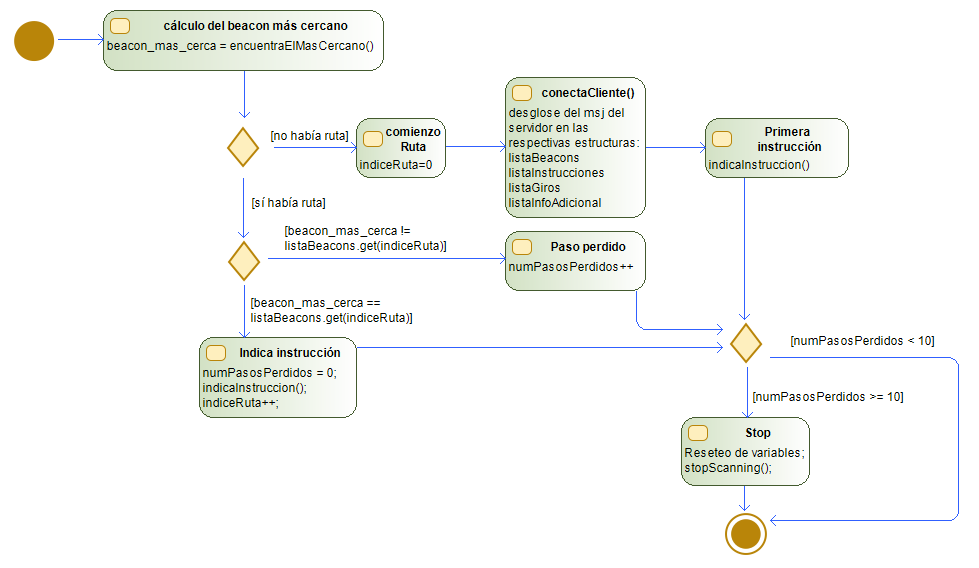
\includegraphics[width=1\textwidth]{Imagenes/Capitulo4/diagramasUML/onEddystonesUpdated}
		\caption{Diagrama de actividad simplificado para la función \textit{onEddystonesUpdated}.}
		\label{fig:diag_clienteSeguimientoRuta}
	\end{figure}
	
\end{itemize}


\section{Adaptación para la reutilización de la aplicación sobre otro edificio}

A lo largo de este capítulo se ha visto la implementación orientada a la Facultad de Informática de la UCM. Sin embargo, no se ha podido realizar un estudio exhaustivo del funcionamiento de la aplicación en esta ubicación debido al estado sanitario de emergencia declarado en febrero de este año 2020 y, su posterior prolongación, hasta final de curso. Así las cosas, se ha tratado de hacer la aplicación lo más genérica posible, de tal manera que, si se quisiera utilizar la tecnología \textit{Bluetooth} para mapear otro espacio, nuestro trabajo pueda ser reutilizado haciendo una cantidad mínima de cambios. A continuación veremos los aspectos que deberían ser modificados.

\subsection{Cambios en el servidor}

El código del servidor se basa, principalmente, en la información del edificio que proporcionan los archivos xml que se vieron en la Sección \ref{sub:mapeo_xml} y el archivo \textit{destinos.json} que se trató en la Sección \ref{sub:func_servidor}. Todos estos archivos deberían ser sustituidos por los correspondientes al nuevo edificio que se desea mapear. Prestando especial atención a los pesos que se colocan en las distintas conexiones de los cuadrantes, pues son claves para el algoritmo de generación de la ruta (ver Sección \ref{sub:rutaOptima}). Así mismo, se debe establecer correctamente el lado del cuadrante en el que se encuentra el punto de interés del mismo (norte, sur, este u oeste), pues de ello dependen las instrucciones que indican al usuario dónde se encuentra el destino o las instrucciones que se dan al usuario tras el cambio de planta, en la zona de los ascensores. De esta manera, si se quisiera utilizar el código del servidor para otro edificio con los mismos requisitos que la Facultad bastaría con sustituir los archivos xml correspondientes al edificio, permitiendo así que no se requieran conocimientos específicos de programación para adaptar el código y facilitando su reutilización.

A pesar de que el código está pensado e implementado para dar servicio a un edificio de características similares a la Facultad de Informática de la UCM también se ha pensado en posibles variantes que podrían surgir a la hora de adaptar el código a otro espacio. A continuación se plantean algunos casos y la solución propuesta: 

\begin{itemize}
	\item En el caso de la Facultad de Informática hemos establecido que cada cuadrante tiene un único punto de interés. Por ejemplo, los cuadrantes de los pasillos tienen un aula como punto de interés, pero podría ocurrir que en otra facultad hubiera aulas a ambos lados del pasillo y fuera, por tanto, necesario que un cuadrante tuviera más de un punto de interés. Esto se resolvería de manera sencilla adaptando la estructura del cuadrante en los archivos xml: incluyendo una etiqueta que estableciera la ubicación de cada punto de interés y adecuando en el código la lectura del mismo. En el archivo \textit{destinos.json} se incluiría una nueva entrada para el destino, de tal manera que tendríamos dos entradas con el mismo cuadrante (esto no supone un problema pues la clave de la tabla hash donde se almacena la información es el nombre del destino y no el cuadrante). Una vez modificados estos archivos bastaría con indicar a la función \textit{genera} cuál es la ubicación del destino dentro de su cuadrante para que indique al usuario la posición del destino correctamente al finalizar la ruta.
	
	\item Otra situación que nos podemos encontrar es aquella en la que la estructura del edificio y los puntos que se quieran mapear se encuentren a una distancia próxima, obligando a que el tamaño de los cuadrantes se vea reducido. En este caso, dar instrucciones al usuario cada cuadrante puede resultar molesto, puesto que se darían instrucciones con demasiada frecuencia. Es por ello que se incluye una variable contador en la función \textit{generar} que permite establecer el número de cuadrantes que queremos ``saltar'' antes de dar una nueva instrucción\footnote{En el propio código se han incluido en comentarios los cambios necesarios para la implementación de esta funcionaliadad.}, siempre que la dirección del usuario se mantenga estable. Es decir, no haya que hacer un giro, pues en ese caso debemos advertir al usuario.
\end{itemize}


%Todos los cambios mencionados, a excepción de los archivos que no forman parte del código, constituyen cambios necesarios para adaptar el edificio a personas con discapacidad visual, puesto que, si la aplicación no estuviera diseñada para ellos no habría necesidad de dar indicaciones tan detalladas.


%\subsection{Cambios en el cliente}

%El cliente es la parte menos dependiente del edificio, puesto que en ningún momento contiene información del mismo, a excepción de la lista de destinos que se incluye tanto en la interfaz como en el archivo \textit{listasStringsApp.xml}. En este archivo se encuentran los destinos con el mismo nombre que el servidor los representa en el archivo \textit{destinos.json}, lo que permite que antes de conectar con el servidor podamos comprobar que el destino es correcto. También habría que modificar esta lista de destinos en las instrucciones de uso de la aplicación para que el usuario pueda acceder a ella sin necesidad de tener que simular el inicio de una ruta.



